\documentclass[twocolumn,superscriptaddress,aps,prb,floatfix]{revtex4-1}

\usepackage{graphicx}% Include figure files
\usepackage{dcolumn}% Align table columns on decimal point
\usepackage{bm}% bold math
\usepackage{color}
\usepackage[caption=false]{subfig} 

\usepackage{listings}

\definecolor{dkgreen}{rgb}{0,0.6,0}
\definecolor{gray}{rgb}{0.5,0.5,0.5}
\definecolor{mauve}{rgb}{0.58,0,0.82}

\lstset{frame=tb,
  language=python,
  aboveskip=3mm,
  belowskip=3mm,
  showstringspaces=false,
  columns=flexible,
  basicstyle={\small\ttfamily},
  numbers=none,
  numberstyle=\tiny\color{gray},
  keywordstyle=\color{blue},
  commentstyle=\color{dkgreen},
  stringstyle=\color{mauve},
  breaklines=true,
  breakatwhitespace=true,
  tabsize=3
}

\usepackage{amsthm}
\usepackage{amsmath}
\usepackage{amssymb}


\newcommand{\figref}[1]{Fig. \ref{#1}}


\newtheorem{theorem}{Theorem}[section]
\newtheorem{lemma}[theorem]{Lemma}
\newtheorem{proposition}[theorem]{Proposition}
\newtheorem{corollary}[theorem]{Corollary}

%\newenvironment{proof}[1][Proof]{\begin{trivlist}
%\item[\hskip \labelsep {\bfseries #1}]}{\end{trivlist}}
%\newenvironment{definition}[1][Definition]{\begin{trivlist}
%\item[\hskip \labelsep {\bfseries #1}]}{\end{trivlist}}
%\newenvironment{example}[1][Example]{\begin{trivlist}
%\item[\hskip \labelsep {\bfseries #1}]}{\end{trivlist}}
%\newenvironment{remark}[1][Remark]{\begin{trivlist}
%\item[\hskip \labelsep {\bfseries #1}]}{\end{trivlist}}

%\newcommand{\qed}{\nobreak \ifvmode \relax \else
%      \ifdim\lastskip<1.5em \hskip-\lastskip
%      \hskip1.5em plus0em minus0.5em \fi \nobreak
%      \vrule height0.75em width0.5em depth0.25em\fi}

\begin{document}

%\allowdisplaybreaks

\title{How nonconvex is it? Exploring neural network geometry through Dynamic String Sampling}


\author{C. Daniel Freeman}
\email{daniel.freeman@berkeley.edu}
\affiliation{Department of Physics, University of California, Berkeley, CA 94720, USA}

\author{Joan Bruna}
\affiliation{Department of Statistics, University of California, Berkeley, CA 94720, USA}


\date{\today}

\begin{abstract}
 The natural tool for understanding neural network training is \emph{nonconvex optimization}.  In practice, this means that, for some given learning task, a loss function is optimized via some flavor of gradient descent.  While this strategy has led to great success, it is surprising that not much is known about the geometry of the loss function itself.  In this manuscript, we examine the geometry of these loss functions for several learning tasks (QUAD, MNIST).  In so doing, we provide both a quantitative handle on problem nonconvexity as well as an algorithm for estimating that nonconvexity (Dynamic String Sampling).  Operationally, given two models which have nearly the same loss $L_0$ on test data, our algorithm searches for continuous paths in the space of model parameters which do not exceed $L_0$.  Whether such a path can be found defines a notion of connectedness, and thus nonconvexity.
\end{abstract}

\maketitle


%%%%%%%%%%%%%%%%%%%%%%
%%%%%%%%%%%%%%%%%%%%%%
\section{Introduction}
\label{sec:Intro}
%%%%%%%%%%%%%%%%%%%%%%
  



	
%%%%%%%%%%%%%%%%%%%%%%
\section{Quantifying Nonconvexity}
\label{sec:QuanNoncon}

\subsection{Definitions}
\label{sec:Defs}
%%%%%%%%%%%%%%%%%%%%%%

 For a model with network parameters $\theta_i$, and a learning problem with sample space $X$, the fundamental object of study is the loss function, $L(X, \theta_i)$.  In practice, one only has access to an estimate of the loss function over some restricted subset, $\chi_i$, of the sample space: $E( L(X, \theta_i), \chi_i )$.  Unless otherwise stated, the loss functions computed throughout are assumed to be on a restricted test set not used during training.
 
 A key ingredient of the algorithm is the use of an \emph{interpolated model}.  For two given models, $\theta_1$ and $\theta_2$, we defined the interpolated model with parameter $t$ as follows:
 
\begin{equation}
\Theta (\theta_1 ,\theta_2, t) := \theta_1 (1-t) + \theta_2 t
\end{equation}

 Thus, the interpolated model parameters---i.e., weights and biases---are simply linearly interpolated between two given models.
 
 Additionally, the algorithm requires an estimate of the interpolated loss curve:

 \begin{equation}
 \gamma(\theta_1, \theta_2) := L (X ,\Theta (\theta_1, \theta_2, t)), t \in [0,1]
 \end{equation}

 or, an estimate of the loss on those models which are linear interpolations sitting between $\theta_1$ and $\theta_2$.  More specifically, we seek efficient estimates of the location of the maxima, $t^* := \frac{d \gamma(\theta_1, \theta_2, t)}{dt} \bigg|_{t^*} = 0, \frac{d^2 \gamma(\theta_1, \theta_2, t)}{dt^2} \bigg|_{t^*} < 0$.  While in principle, the interpolated loss curve could have rich structure, in practice it is generally fairly smooth, thus straightforward hill climbing algorithms can efficiently locate these points.
 
 Finally, for a pair of models $(\theta_1, \theta_2)$, it will be convenient to define the maximum interpolated error:
 
  \begin{equation}
  \Gamma(\theta_1, \theta_2) := \rm{min}_{\Theta^*(\theta_1, \theta_2)}\:\rm{max}\:L (X, \theta_i) \bigg|_{\theta_i \in \Theta^*} \label{eq:minmaxerror}
  \end{equation}
 
 where $\Theta^* (\theta_1, \theta_2)$ is \emph{any} continuous path in the space of weights connecting $\theta_1$ and $\theta_2$.  Thus, $\Gamma(\theta_1, \theta_2)$ represents the minimum possible maximum loss achieved by those paths in the space of weights connecting $\theta_1$ and $\theta_2$.  More intuitively, if $\Gamma (\theta_1, \theta_2) \leq \rm{max}\: (L(X,\theta_1), L(X,\theta_2))$, then the models are ``connected''---there exists a continuous path in the space of models with total loss never exceeding the maximum loss achieved by $\theta_1$ or $\theta_2$. 
 
 \subsection{The Algorithm}
 \label{sec:Alg}
 
 1. Train two models $\theta_i$ and $\theta_j$ to a threshold loss value, $L_0$.
 
 2. Determine the location of the global maxima, $t^*$, on the interpolated loss curve $\gamma(\theta_i, \theta_j)$. 
 
 3. Perform gradient descent on the interpolated model $\Theta (\theta_i, \theta_j, t^*) := \theta_{i,j}$ until it is below $\alpha L_0$ for some $\alpha \in [0,1]$ .
 
 4. Calculate the maxima of the interpolated losses $\gamma(\theta_i, \theta_{i,j})$ and $\gamma(\theta_{i,j}, \theta_j)$.  If these maxima are below $L_0$, then stop recursing on this branch and proceed to remaining branches(see 5).  If not, proceed to step 5.
 
 5. For those pairs, $\theta_a, \theta_b$ from step 4 for which the maxima exceeds $L_0$, start a new branch by returning to step 2 and making the replacement $i->a$ and $j->b$.  If depth exceeds $d$, stop (see below).
 
 \begin{figure}
\begin{center}
\scalebox{1}{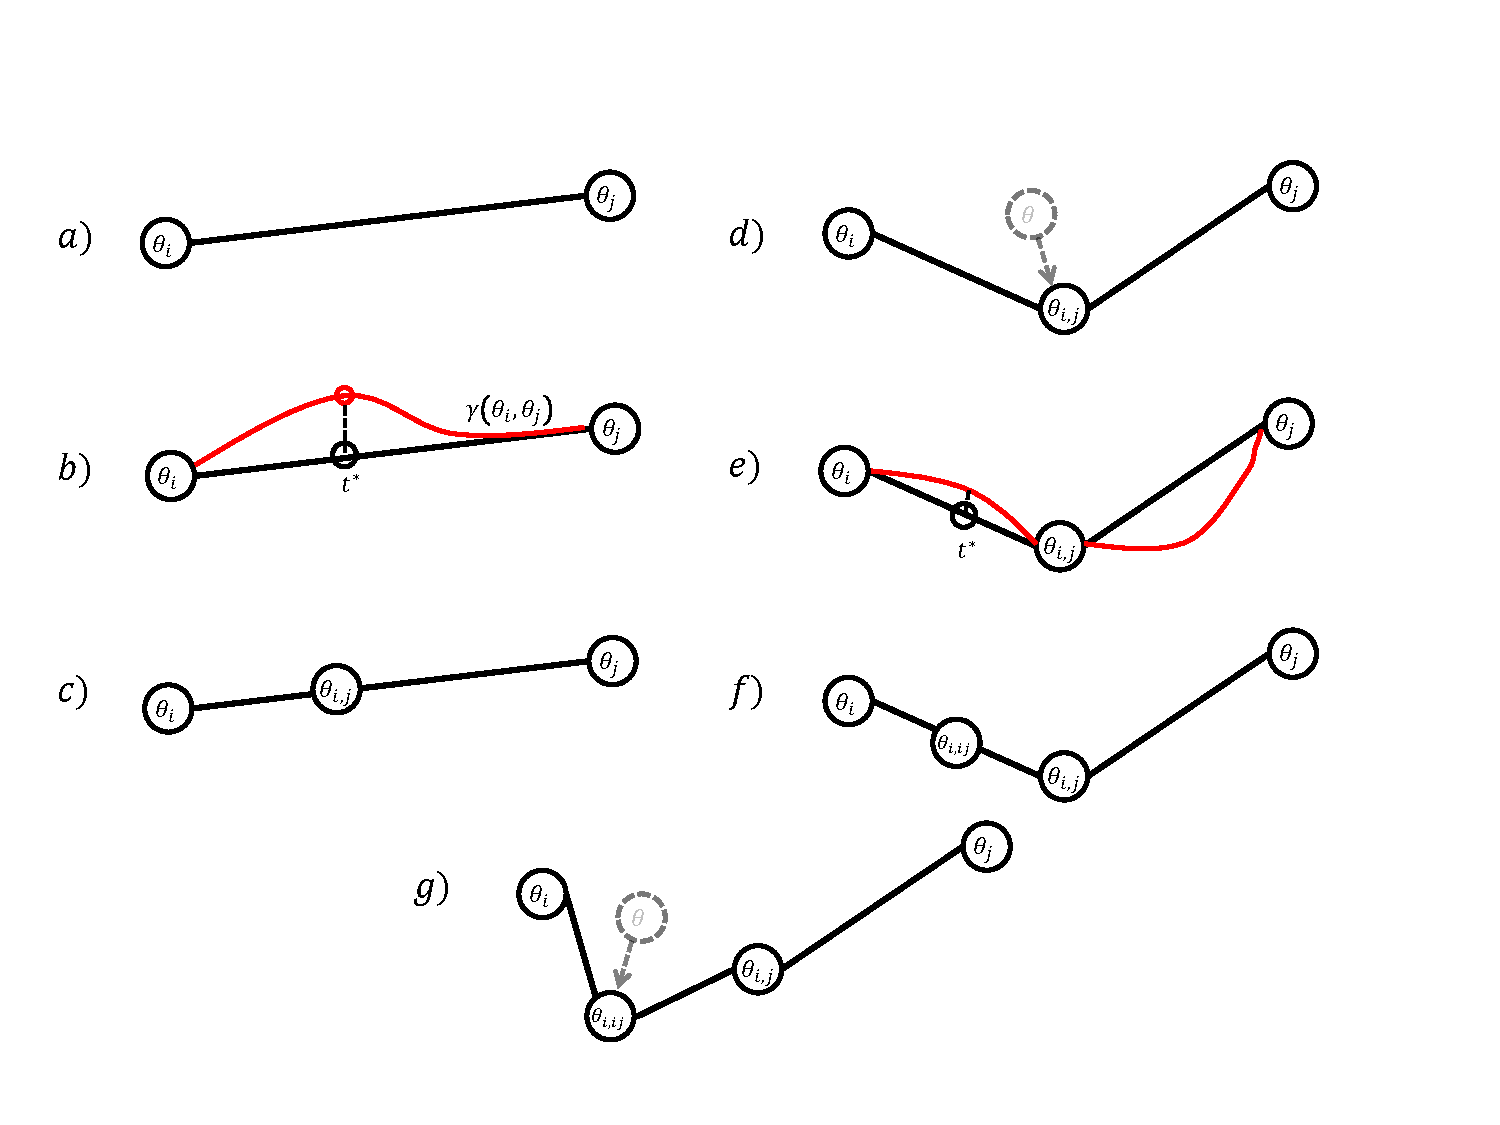
\includegraphics[width=1.0\columnwidth]{AlgorithmFigure}}
\end{center}
\caption{A cartoon of the algorithm.  $a):$ The initial two models with approximately the same loss, $L_0$. $b):$ The interpolated loss curve, in red, and its global maximum, occuring at $t=t^*$. $c):$ The interpolated model $\Theta(\theta_i, \theta_j, t^*)$ is added and labeled $\theta_{i,j}$.  $d):$ Stochastic gradient descent is performed on the interpolated model until its loss is below $\alpha L_0$. $e):$ New interpolated loss curves are calculated between the models, pairwise on a chain.  $f):$ As in step $c)$, a new model is inserted at the maxima of the interpolated loss curve between $\theta_i$ and $\theta_{i,j}$.  $g):$  As in step $d)$, gradient descent is performed until the model has low enough loss.}
\label{fig:AlgorithmFigure}
\end{figure}
 
 We provide a cartoon of the algorithm in \figref{fig:AlgorithmFigure}.  If the algorithm succeeds, then the output of the algorithm is a sequence of models, $\theta_i$ such that the pairwise interpolated loss curve between each in a sequence will be less than the threshold $L_0$.  Thus, the algorithm outputs a continuous path in parameter space connecting the original two models such that everywhere along the path, the total loss is less than or equal to the loss of the original models.
 
 As written, if a path does \emph{not} exist, then the algorithm will clearly not converge.  Thus, on top of the parameter $\alpha$, discussed below, the algorithm has an additional free parameter in the \emph{depth} chosen to explore.  For convenience, we define the string of models produced by the algorithm at depth $d$ with parameter $\alpha$ to be the \emph{interpolated string}, $S(\theta_1, \theta_2, \alpha, d)$.  These are precisely those models recursively generated by the algorithm in step 3.  Further, these models are naturally ordered along a path, starting from $\theta_1$ and terminating on $\theta_2$, as indicated in \figref{fig:AlgorithmFigure}.
 
 Finally, to use this as a tool to diagnose convexity, we define the \emph{maximum interpolated error at depth $d$ and tolerance $\alpha$}:
 
 \begin{align}
 \tilde{\Gamma}( \theta_1, \theta_2, d, \alpha ) &:= \rm{max}\ \gamma(\theta_i, \theta_j, t)\\ \notag
 &i,\ j\ \rm{neighbors\ in}\ S(\theta_1, \theta_2, \alpha, d)
 \end{align}
 
 where by ``neighbors in $S(\theta_1, \theta_2, \alpha, d)$'', we only mean that the models are immediately adjacent on the interpolating string.  This quantity upper bounds the true maximum interpolated error, i.e. \eqref{eq:minmaxerror}.
 
 In summary: the algorithm recursively produces and trains new models lying on a continuous path in the space of model parameters, i.e. a string.  Training via gradient descent biases the path towards valleys on the loss surface, thus encouraging the loss along this path to be low.  In practice, the parameter $\alpha$ is chosen to be less than 1 to aid convergence.  We provide numerical and theoretical evidence for this choice in section SECTIONGOHERE.
 


 %%%%%%%%%%%%%%%%%%%%%%
\section{Analytic Toy Model}
\label{sec:ToyModel}

 To build intuition for the nonlinear case, here we treat an ``almost linear'' regression task.  The strategy will be first, to understand how dynamic string sampling applies in an analytically tractable model, and second, to leverage this intuition for the more complicated numerical systems to follow.  We will proceed by studying the level sets of the \rm{QUARTICLOSS} toy model defined as followed:
 
 For weight matrices $w_1, w_2$, input column vectors $x_i$ of dimension $d_1$, and output scalars $y_i$, suppose we aim to minimize the loss function
 
  \begin{equation}
 L(w_1,w_2)=(w_1 w_2 x - y)^2 \label{eq:losseq}
  \end{equation}
 
 For simplicity, suppose $w_1$ is a row vector with dimension $d_2$.  This fixes the dimension of $w_2$ to $d_1$ by $d_2$.
 
 Suppose we are given the globally optimal $w_1^*$ and $w_2^*$ which minimize $L$.  These weights are not unique, because we can reparameterize the global optima in the following way:
 
  \begin{align}
 w_1^* &\rightarrow \rm{any\ nonzero\ vector} = w_1 \\
 w_2^* &\rightarrow \frac{w_1^T}{||w_1||} a^* + \alpha (w_1^T)_\perp a^*
  \end{align}
  
  where $a^*$ is the row vector $a^*=w_1^* w_2^*$ which globally optimizes \eqref{eq:losseq}, and $\alpha$ is an arbitrary scalar.  This freedom represents an internal symmetry of the weights.
  
  Given two models $w_1^A w_2^A = a^*$ and $w_1^B w_2^B = a^*$, let $w_1^A \cdot w_1^B=||w_1^A||||w_1^B||\rm{cos}\theta$.  Either can be continuously connected to the other via the following two steps.  Without loss of generality, we will connect the $A$ components to the $B$ components.  First, the component of $w_2^A$ perpendicular to $w_1$ is scaled linearly from its original value $\alpha$ to $\alpha^*$:
  
 \begin{equation}
 w_2^A = \frac{w_1^T}{||w_1||} a^* + (w_1^T)_\perp a^* \rightarrow \frac{w_1^T}{||w_1||} a^* + \alpha^* (w_1^T)_\perp =: w_2^{**}
  \end{equation}
  
 Where $\alpha^*=\frac{1-||w_1^B||\rm{cos}\theta}{||w_1^B|| \rm{sin}\theta}$.  Defined in this way, $w_2^{**}$ now satisfies both $w_1^A w_2^{**} = a^*$ as well as $w_1^B w_2^{**} = a^*$.  Then, simple linear interpolation connects $w_1^A$ to $w_1^B$:
 
  \begin{equation}
 w_1^a \rightarrow w_1^a (1-t) + w_1^b t
  \end{equation}
  
  Thus, linearly scaling first $\alpha$ to $\alpha^*$ and then scaling $t$ from $0$ to $1$ connects $w_1^A$ to $w_1^B$.  Crucially, the entire procedure preserves the global minimum of the loss function.  
  
  Now that we have shown a continuous path exists for this internal symmetry, it remains to be shown that DSS will faithfully produce a continuous path.  For DSS, the relevant interpolation equations are:
  
  \begin{align}
  w_1(t) &= w_1^A (1-t) + w_1^B t
  w_2(t) &= w_2^A (1-t) + w_2^B t
  \end{align}
  
  Examining $w_1(t) w_2(t)$, the first and last terms in the product yield $(1-t)^2 a^* + t^2 a^*$.  The remaining cross terms can be rewritten as $\gamma t(t-1) a^*$ for a constant $\gamma$.  Because we are promised that $A$ and $B$ are global minima in the space of weights, the loss is either constant along the path, or reaches a reaches a global maxima somewhere, which we call $t^*$.  In the former case, we are done, because DSS will have provided a continuous path in the space of weights with nonincreasing loss.
 
  In the latter case, 
 
 
 
 %%%%%%%%%%%%%%%%%%%%%%
\section{Numerical Experiments}
\label{sec:NumExp}

For our numerical experiments, we aimed to extract qualitative features of both small, toy networks, as well as of larger workhorse networks suitable for use on real world tasks (e.g. MNIST).  At its core, the maximum interpolated error (i.e., \eqref{eq:minmaxerror}) is a measure of problem nonconvexity---or, more precisely, of the nonconvexity of the loss surface of a given architecture on a particular learning problem.


\subsection{Polynomial Regression}
\label{sec:PolyFuncs}
%%%%%%%%%%%%%%%%%%%%%%

 Polynomial function regression is a task for which small neural networks can achieve extremely high accuracy.  For our numerical experiments, we studied a 1-4-4-1 fully connected multilayer perceptron style architecture with RELU activation and RMSProp optimization.  For ease-of-analysis, we restricted the family of polynomials to be strictly contained in the interval $x\in[0,1]$ and $f(x)\in[0,1]$.
 
 Discussion of different Loss functions
 
 etc.


%%%%%%%%%%%%%%%%%%%%%%
\subsection{MNIST}
\label{sec:MNIST}
%%%%%%%%%%%%%%%%%%%%%%


%%%%%%%%%%%%%%%%%%%%%%
%%%%%%%%%%%%%%%%%%%%%%
\section{Discussion}
\label{sec:Discussion}
%%%%%%%%%%%%%%%%%%%%%%

 
 

\bibliography{nonconvex}

\end{document}
%
% {**}{**}{**} End of file apssamp.tex {**}{**}{**}
